\section{Dynamic VMPP Algorithms}
\label{sec:vm-schedulers}
\vspace*{-.2cm}
To illustrate the interest of \vmps, we implemented three dynamic VM
placement mechanisms: a centralized one based on the Entropy
proposal~\cite{Hermenier:2009:ECM:1508293.1508300}, a hierarchical one
based on Snooze~\cite{feller:ccgrid12}, and a fully-distributed one
based on DVMS~\cite{quesnel:cpe2012}.
%\MS{We should differentiate more clearly between the complete VMPP
 % system and the solver.}
%
These systems enable, if it is possible,  the resolution  of violations in form of
overloaded nodes. A host is overloaded when the VMs try to consume
more than 100\% of the CPU capacity of the host. In such a case, a
resolution algorithm looks for a reconfiguration plan that can lead to
a viable configuration. For the sake of
simplicity, we chose to use the latest solver developed as part of the Entropy
framework~\cite{hermenier:cp11} in the three systems as this resolution algorithm.
The Entropy solver evaluates different viable configurations until  it
reaches a predefined timeout.
% Giving up consolidation optimality in favor of scalability, this
% algorithm provides a ``repair mode'' that enables the correction of VM
% requirement violations. The optimal solution is a new placement that
% satisfies the requirements of all VMs while minimizing the cost of the
% reconfiguration.
Once the timeout has been triggered, the algorithm returns the best
solution among the ones it finds and applies the associated
reconfiguration plan by invoking live migrations in the simulation
world.
%
% Although using the Entropy VMPP solver implies a modification from the
% original Snooze proposal, we highlight that our goal is to
%
% and thus we believe that such a modification is acceptable as it
% does not change the global behavior of Snooze

%Simulating these three VMPP systems illustrates the capabilities of
%\vmps. Moreover, by conducting such a comparison, we also investigate
%the pros and cons of the three architecture models on which these
%proposals rely on.% (\ie centralized, hierarchical and distributed).

In the remainder of this section, we present an overview of the
three systems, showing, in particular, that the extended abstractions
for hosts (\texttt{XHost}), VMs (\texttt{XVM}) and the functions of
the \sg MSG API enabled us to develop them in a direct and natural
manner.

%\subsection{Entropy-based Centralized Approach}
\paragraph{Entropy-based Centralized Approach}
\label{subsec:entropy}
The centralized VM placement mechanism consists in one single \sg
process deployed on a service node. This process implements a simple loop that
iteratively checks the viability of the current configuration by
invoking the aforementioned VMPP solver with a predefined
frequency.
% $p$ is defined as an input parameter of the simulation.
% \AL{Should we explain the issue right now or not if we add VMPP section}
% Indeed, during
% the computation and the application of a schedule, the algorithm does
% not enforce QoS properties anymore, and thus cannot react quickly to
% violations. Second, since the manipulation of VMs is costly, the time
% needed to apply a new schedule is particularly important: The longer
% the reconfiguration process is, the higher is the risk that the schedule may
% be outdated, due to the workload fluctuations, when it is eventually
% applied.
% \vmps enables researchers to investigate such concerns in-depth.
%
% As the Entropy proposal does not provide a specific mechanism for the
% collection of resource usage information but simply uses an external
% tool (namely ganglia), we had two different ways to implement the
% monitoring to process: either by implementing additional asynchronous
% transmissions as a real implementation of the necessary state updates
% would proceed or, in a much more lightweight manner,
The resource usage is monitored through direct accesses
% by the aforementioned process
to the states of the hosts and their respective VMs.
%, while accounting for communication overheads explicitly.
%\AL[MS]{Not sure I understood  what you would say ?}
% induced by communication in the ``real'' implementation, for
% instance, can be easily added as part of the lightweight
% simulation. We have implemented this lightweight variant for the
% monitoring
%
% Regarding fault tolerance, similarly to the Entropy proposal, our
% implementation does not provide any failover mechanism.
%
% as mentioned in Section \ref{subsec:traces-analysis},
We also monitor, for each iteration, whether the VMPP solver succeeds
or fails. In case of success, \vmps records the number of migrations
that have been performed, the time it took to apply the
reconfiguration and whether the reconfiguration
led to new violations.

%\subsection{Snooze-based Hierarchical Approach}
\paragraph{Snooze-based Hierarchical Approach}
\label{subsec:snooze}
\AL[MS]{1.5 pages}

We now present the Snooze framework for VM
management~\cite{feller:ccgrid12} as a second case study of how
to implement and simulate advanced algorithms.

\subsubsection{Overview}

We first briefly present the Snooze architecture summarizing its main
characteristics from its presentation~\cite{feller:ccgrid12} and
additional info stemming from personal communications of the Snooze
developers and its implementation~\cite{snoozedev14,snoozeweb}.
\begin{figure}
  {\centering ~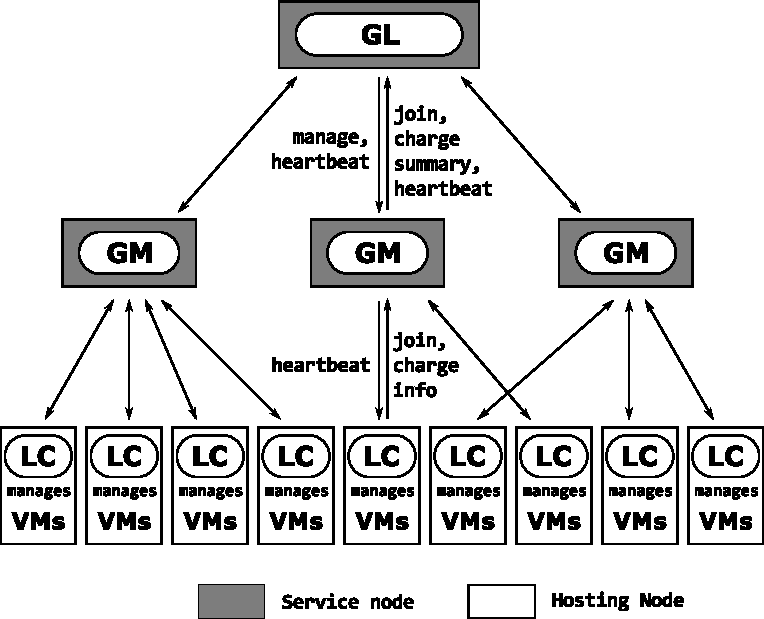
\includegraphics[width=.95\linewidth]{figures/snoozearch.pdf}}
  \caption{Overview of Snooze's architecture}
  \label{fig:snoozearch}
\end{figure}

\paragraph{Architecture}

Snooze harnesses a hierarchical architecture in order to support load
balancing and fault tolerance, see Fig.~\ref{fig:snoozearch}. At the
top of the hierarchy, a \emph{group leader (GL)} (that is installed on
a service node in our simulation) centralizes information about the
whole cluster by keeping summary information about all \emph{group
  managers (GMs)} (also installed on service nodes in our simulation)
that constitute the intermediate layer of the hierarchy. GMs manage a
number of \emph{local controllers (LCs)} (installed on an ordinary
node) and manages the VMs assigned to that node. During execution,
higher-level components periodically send heartbeats to lower-level
components; monitoring information, \eg on the system load, is also
sent periodically in the opposite direction. In order to propagate
information down the hierarchy, Snooze relies on hardware support for
multicast communication. Finally, a number of replicated entry points
allows clients to contact the GL, \eg in order to submit new VMs for
integration into the system.

\paragraph{Algorithms}
\label{sec:snoozeAlgs}

Apart from the handling of faults (described below), two types of
algorithms are of major importance for the administration of the
Snooze architecture: the algorithms that enable components to
dynamically enter the system and the algorithms that propagate info
between the components.

A GL is created, if it does not exist, by promotion of a GM that is
selected according to some leader election algorithm. When a GM joins
a cluster, it starts listening on a predefined channel for the
heartbeat of the GL and registers once it has received the
heartbeat. New LCs first also wait for the GL heartbeat, request a GM
assignment from the GL and register at the GM assigned to them.

Information that is passed within the system consists in periodic
heartbeat message from the GL, GMs and LCs as well as, also periodic,
charge information from LCs sent to their respective GMs and summary
charge info sent by GMs to the GL.


\paragraph{Fault tolerance}

GLs, GMs and LCs may fail during the system execution. System
components identify that a node on the corresponding higher-level node
has failed (the GL in case of a GM, a GM in the case of an LC) in an
asynchronous fashion through the lack of heartbeat messages.

In the case of a GL failure, one of the GMs becomes the new GL, stops
its GM activities and prevents the LCs it manages so that they can
start rejoining the system. If a GM fails, the GL and the LCs it has
managed will become aware of it based on the lack of heartbeats,
update its data structures and, for the LCs, rejoin the system. If an
LC fails, its GM will finally learn of it due to the missing heartbeat
and charge information of the LC. The GM will then remove the LC from
its data structures.

\subsubsection{Simulation using Simgrid}

Snooze can be simulated using our model and tool support in a direct
and natural manner. The extended abstractions \MS[MS]{Refer to
  Sec.~\ref{sec:overview}} for hosts (\texttt{XHOST}) and VMs
(\texttt{XVM}) provide low-level facilities for scheduling algorithms
that facilitate the implementation of the Snooze simulation. We have
harnessed these facilities in order to implement core characteristics
of Snooze: the monitoring of all VMs that are part of an LC and the
migration of all VMs of the set of LCs that are managed by a GM.

The remaining concepts and algorithms of Snooze are implemented using
means of our framework, the facilities provided by Simgrid and
standard Java mechanisms. Communication between Snooze actors is
implemented based on Simgrid's primitives for, mainly asynchronous,
event handling; in particular, hardware-supported multicast
communication that is used, for example, in order to relay heartbeats
is implemented as a dedicated actor that manages a state representing
GL and GM heartbeat groups and relaying heartbeat events.

The Snooze simulation uses, as its original counterpart, a
multi-threaded implementation in order to optimize reactivity even for
large groups of LCs (or GMs) that have to be managed by one GM (or
GL).

\subsubsection{Variants}
\label{sec:snoozeVariants}

Our simulation framework facilitates the simulation of variants of
placement algorithms. In the following, we present three non-trivial
variants that we have implemented and explored: a variant of the
assignment algorithm of LCs to GMs, periodic vs.\ reactive scheduling,
and a variant of the algorithms of how GMs and LCs join the system.


\paragraph{Assignment of LCs to GMs}

LCs are assigned to GMs by the GL as part of the LC join protocol. In
Snooze's native implementation LCs are assigned in a round-robin
fashion to the known GMs. If GMs join (and leave) the system at the
same time as LCs, a round-robin strategy at join time, however, does
not ensure an even distribution. This may happen, for instance at
startup time of the system, when new GMs and LCs enter the system, or
in case of failures, which trigger GM and LC joins. In order to
evaluate the imbalance resulting from a round-robin strategy (as well
as others) we have implemented the LC assignment protocol in a modular
fashion and applied it in diverse highly-dynamic settings in which GMs
and LCs enter the system at the same time. Furthermore, we have
implemented a best-fit strategy that assigns LCs to GMs with minimal
load or to GMs with the smallest number of assigned LCs (if several
GMs with minimal load exist). The best-fit strategy can significantly
improve the scheduling characteristics of hierarchical placement
algorithms as shown by the experimental data presented in
Sec.~\ref{sec:snoozeVariantsEval}. Furthermore, it should always be
at least as good as the round-robin strategy (the corresponding proof
is left to future work).


\paragraph{Periodic vs.\ reactive scheduling}

Snooze~\cite{feller:ccgrid12} schedules VMs in a periodic fashion:
after a fixed time period a GM calls the scheduler in order to resolve
resource conflicts among the LCs it manages. The information whether a
resource conflict has to be handled is taken based on the summary
information that is periodically sent by the LCs to the GM.

We have provided an alternative, reactive, strategy to scheduling: as
soon as they occur, LCs avert their GMs of resource conflicts; the GMs
then initiate scheduling. Implementing this reactive scheme can be
done using our framework in two manners: either by implementing
additional asynchronous transmissions as a real implementation of the
necessary state updates would proceed or, in a much more lightweight
manner, through direct accesses by the GMs to the states of their
respective LCs. While the latter does not mimic a real implementation
closely, it can be harnessed to yield a valid simulation: delays
induced by communication in the ``real'' implementation, for instance,
can be easily added as part of the lightweight simulation. We have
implemented this lightweight variant of reactive scheduling.


\paragraph{Variants of the join algorithms}

The join algorithms, see Sec.~\ref{sec:snoozeAlgs}, are crucial to the
correctness of Snooze for two main reasons: (i) they have to be
efficient because they can easily form a bottleneck if large numbers
of LCs (GMs) have to be registered at a GM (LC); (ii) they are
multi-phase protocols whose correctness especially in the presence of
faults is difficult to ensure.

In order to investigate the corresponding trade-offs, we have used our
framework to implement join algorithms that may be interrupted at any
time, repeat the the on-going phase a number of times before
reinitiating, if necessary, the entire protocol. Furthermore, the join
protocol is parameterized, \eg, in the number of threads used to
handle registration requests.

Finally, our framework has enabled us to test another aspect of
Snooze's join algorithm as presented by
Feller~\etal.~\cite{feller:ccgrid12},
\MS[MS]{If we succeed to perform the experiment comparing both
  approach, this paragraph should be highlighted.}
a strategy we call the GM rejoin
strategy (GRJ): all GMs should rejoin if a new GM enters the
system. While GRJ supports a form of load balancing (because all LCs
are reassigned to the new set of GMs), our simulation has shown that
this strategy significantly increases the time necessary for
registering GMs and LCs compared to a simpler strategy that does not
modify existing GMs in case a new GM enters the system. This handicap
is particularly pronounced if joins of GMs may be interrupted due to
faults. Concretely, experiments involving 20 GMs and 200 LCs have
shown that this strategy often multiplies the time necessary to join
all 220 components by 10 or more compared to the simple join
strategy. While the qualitative result that the more complex strategy
presented in the paper results in a more time-consuming join process
is not very surprising, the extent of the resulting degradation was
surprising.



%%% Local Variables:
%%% mode: latex
%%% TeX-master: "main"
%%% End:


%\subsection{DVMS-based Distributed Approach}
\paragraph{DVMS-based Distributed Approach}
\label{subsec:dvms}
% TODO Not adressed
%\AL[AL]{Check who write that part, If Flavien did it, then add him as
%  an author}
% As the third use-case, we have implemented the
DVMS (Distributed Virtual Machine Scheduler)~\cite{quesnel:cpe2012} enables the
cooperative and fully-distributed placement of
VMs. A DVMS agent is deployed on each node in order to manage the VMs on
the node and collaborate with (the agents of) neighboring nodes.
Agents are defined on top of an overlay communication network that
defines the node-neighbor relation.
% and can be structured (using, \eg
% Chord~\cite{stoica:2001:sigcomm01}) or unstructured.  For this
% study,
We have implemented a simple % but effective
unstructured overlay that enables the agents to collaborate
% without side effects: when necessary, \eg in case of node failures,
% the overlay
by providing a link to a neighbor %of a node
on the latter's request.
% \MS[AL, JP]{A bit short. What about an architecture figure (as for
%  Snooze?)}




% \paragraph{Iterative Scheduling Procedure.}
% \label{sec:ISP}
% \AL[MS,JP]{if we succeed to have only one or two subsections in
%   Snooze, we should do the same here.}

Fig. \ref{fig:dvms_pte} depictes the DVMS algorithm.
When a node N\(_{\textit{i}}\) detects that it cannot provide enough
resources for its hosted VMs, %(\ie VMs hosted on the server require more
%resources than available),
an \emph{Iterative Scheduling Procedure
  (ISP}) is started:
%
%When a node N\(_{\textit{i}}\)
%detects that it cannot provide enough resources for its hosted VMs,
it initiates a partition, reserving itself to solve the problem (sse
Fig.~\ref{fig:dvms_pte_1}).
Then, its
closest neighbor % , as defined by the network overlay,
is considered.
%
%
%
If this neighbor, N\(_{\textit{i+1}}\),
is already part of another partition, the next neighbor is considered.
%\AL[MS]{Not clear enough, its next neighbor ?}
Otherwise, N\(_{\textit{i+1}}\)
joins the partition (see Fig.~\ref{fig:dvms_pte_2}) and becomes the
partition leader.
% % If the partition is not valid anymore (\eg because the workload of the
% % partition's VM has decreased), N\(_{\textit{i+1}}\)
% % cancels the reservations, destroys the partition and thus frees its
% % nodes for another problem solving procedure.
% % %
% % On the contrary, if the procedure is still valid, N\(_{\textit{i+1}}\)
% % notifies members of the partition that it has become the new
% % leader.
%
The other nodes involved in the partition then send it information about their
capacities and current load. The leader, in turn, starts a scheduling
computation looking for a reconfiguration within the current
partition. If no solution is found, the same algorithm is applied to
the next node N\(_{\textit{i+2}}\).
%
% % In the extreme case a partition may grow until all resources in a
% % cluster contribute to the resolution of its resource scheduling
% % problem.
This approach constructs small parititions in a highly parallel
manner (Fig.~\ref{fig:dvms_pte_3}), thus significantly accelerating
the scheduling process and thus the reactivity criteria.

Most of the DVMS code has been coded in SCALA leveraging the Java
primitives of \sg for the communications between the different DVMS agents.

\begin{figure}[t]
\vspace*{-.6cm}
\subfigure[]{
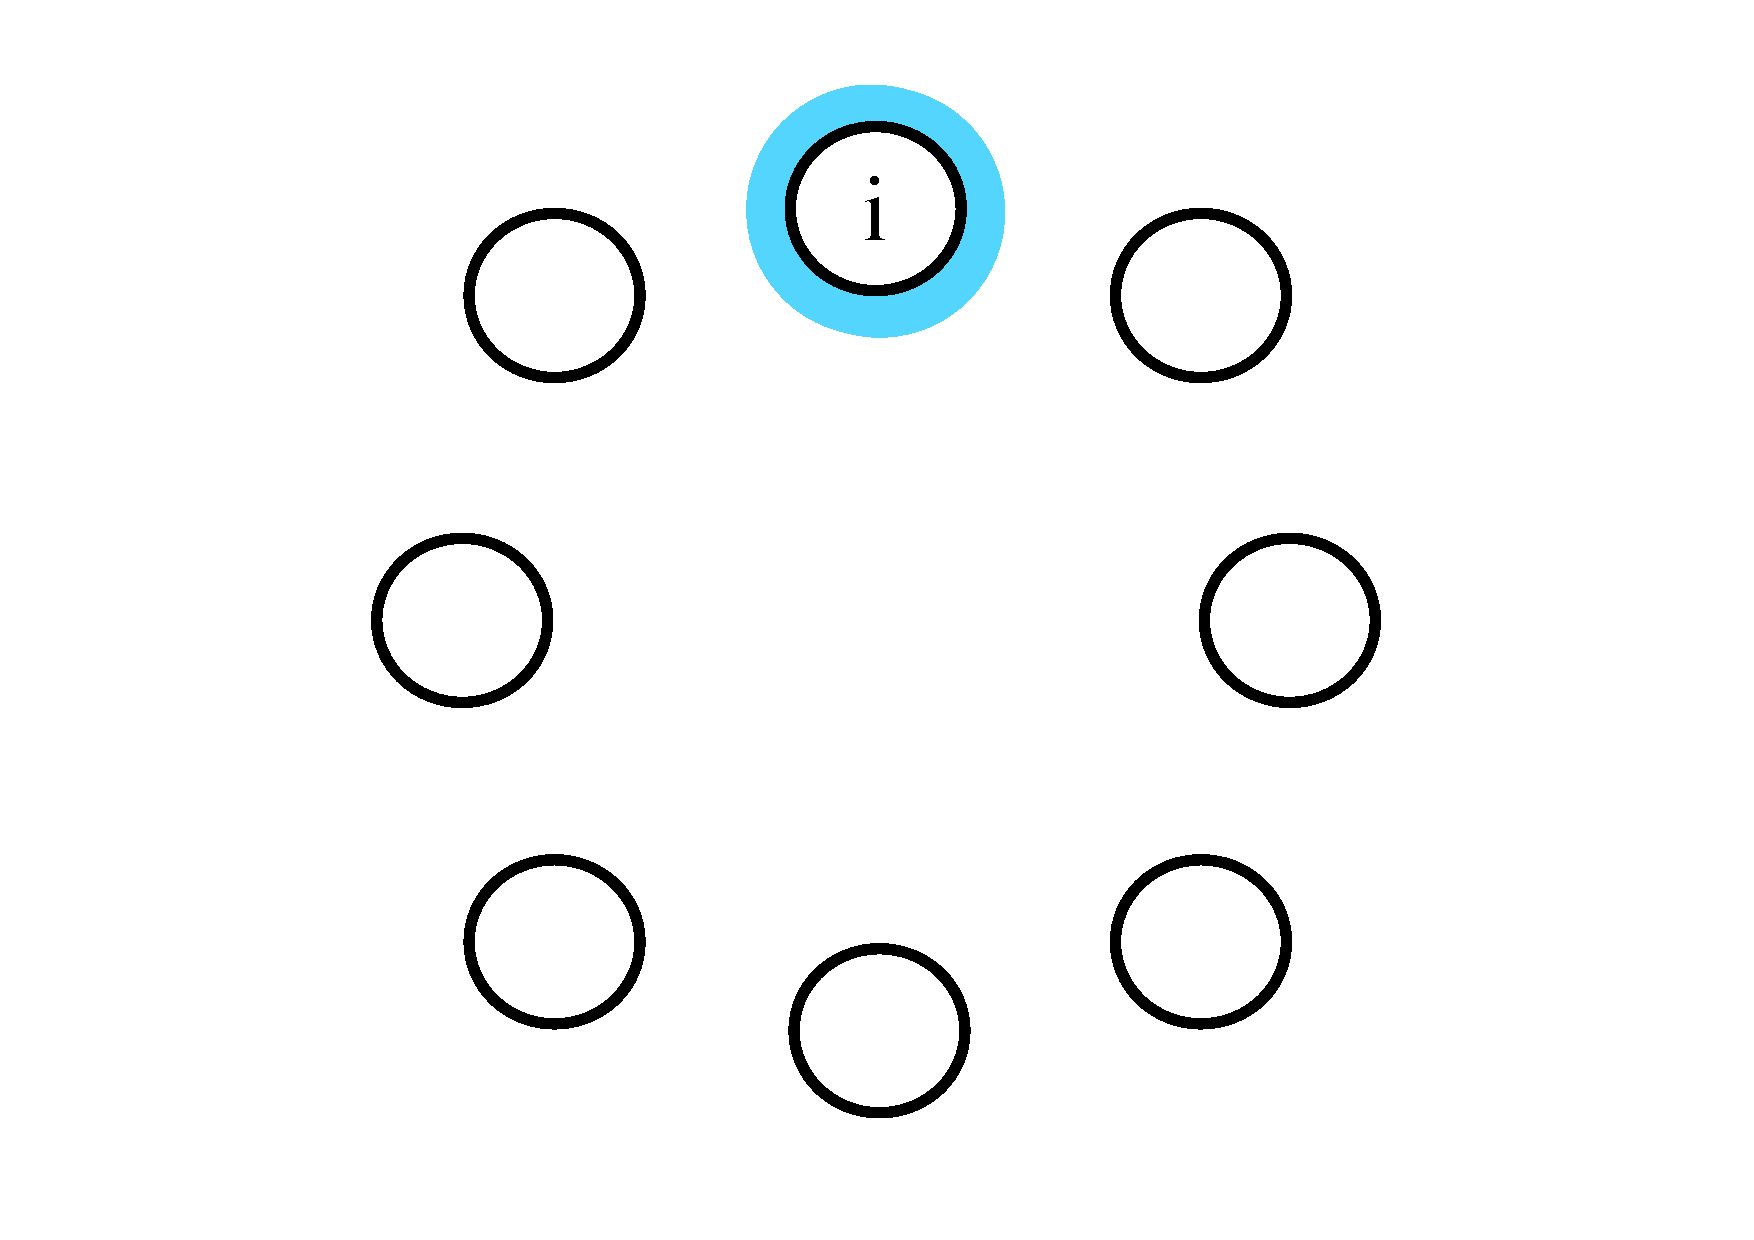
\includegraphics[width=2.7cm]{./figures/fig-24.pdf}
\label{fig:dvms_pte_1}}
%
\subfigure[]{
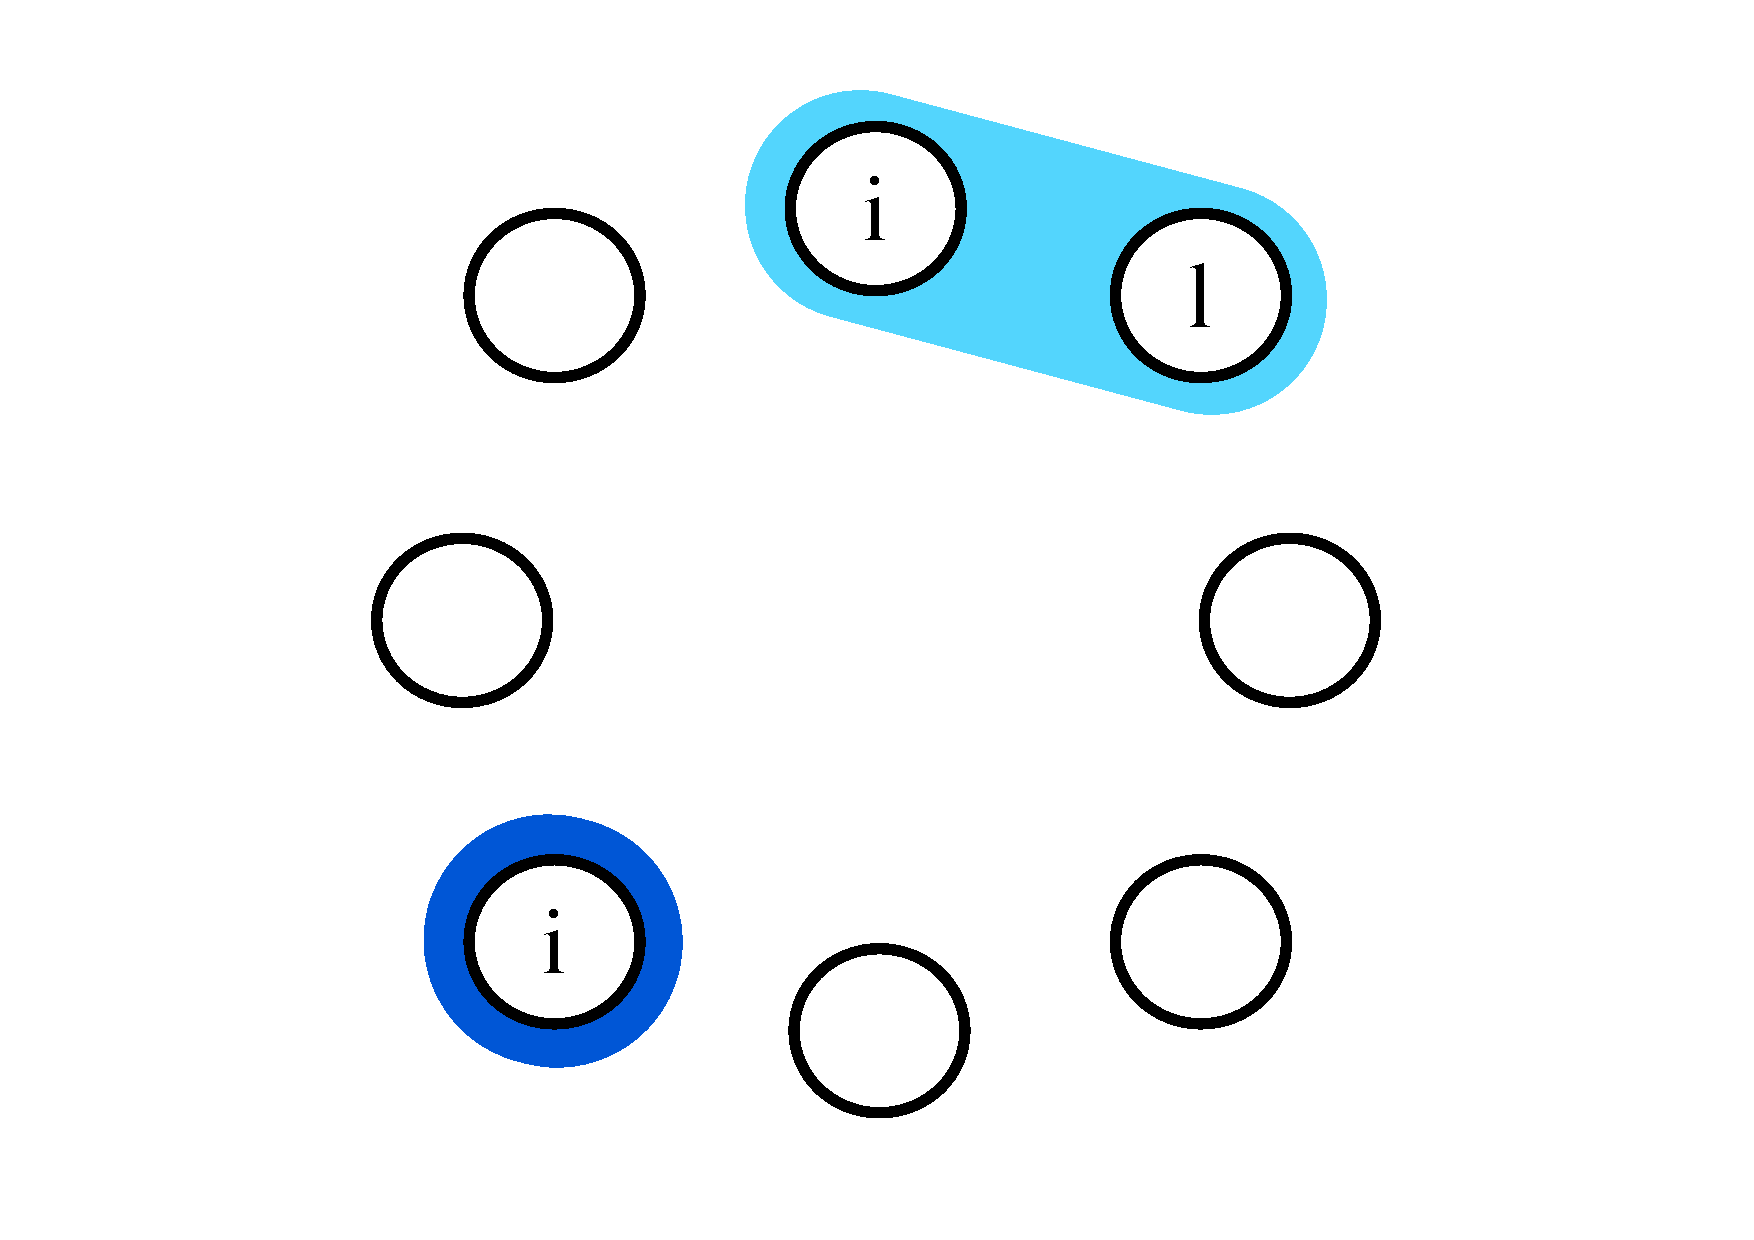
\includegraphics[width=2.7cm]{./figures/fig-25.pdf}
\label{fig:dvms_pte_2}}
%
\subfigure[]{
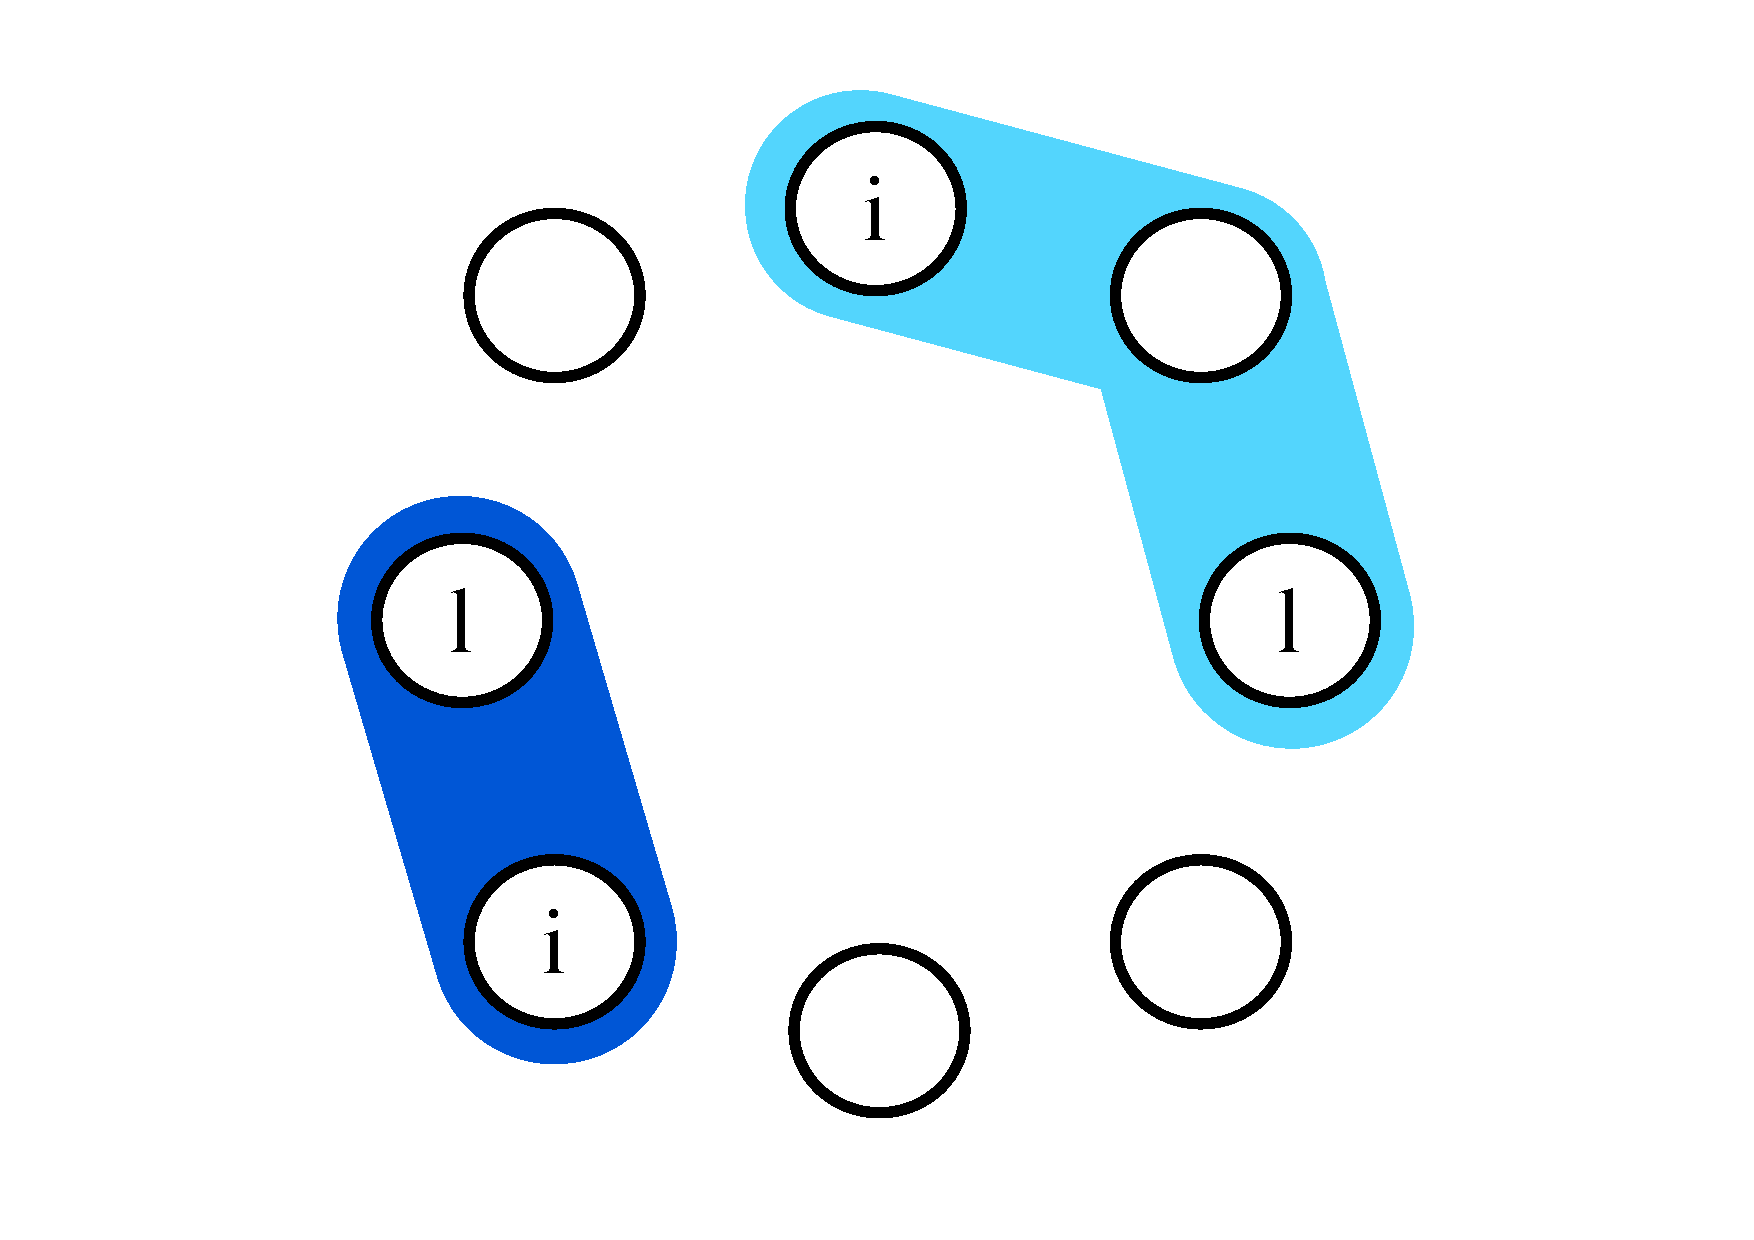
\includegraphics[width=2.7cm]{./figures/fig-26.pdf}
\label{fig:dvms_pte_3}}
%
\subfigure[Legend]{
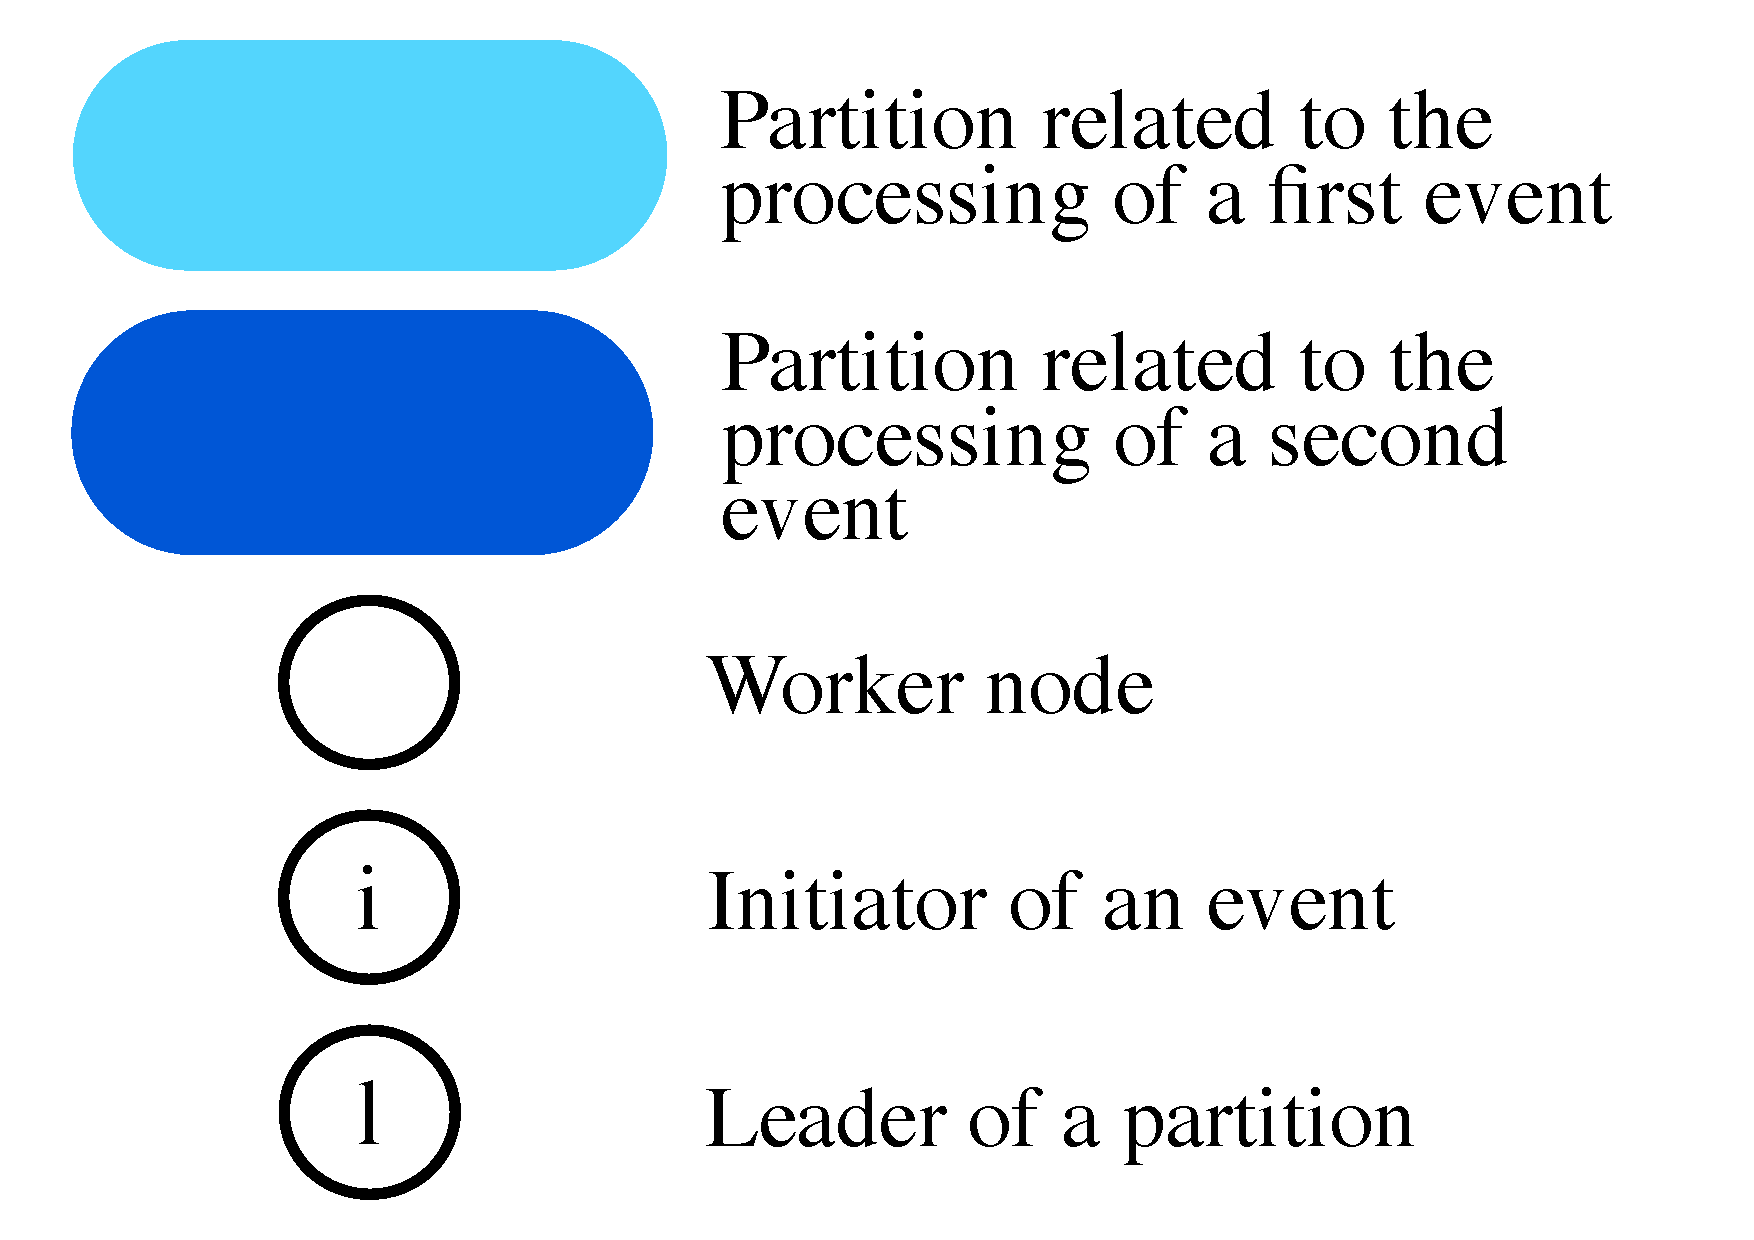
\includegraphics[width=2.7cm]{./figures/fig-27.pdf}
\label{fig:dvms_pte_4}}
%
\vspace*{-.3cm}
\caption{Processing two events simultaneously\label{fig:dvms_pte}}
\vspace*{-.6cm}
\end{figure}


% \subsubsection{Fault-tolerance}

% The main advantage of using overlay networks is that they have
% built-in fault tolerance mechanisms. DVMS therefore works on top of an
% overlay network such as Chord: when a node needs to rebalance its VMs
% workload, it uses the overlay network to find collaborators. For this
% study we implemented a simple overlay network as a flat list of
% agents: a typical request for collaborators includes the list of
% agents that are already collaborating with the requesting agent. A
% link to a new collaborator is then provided to the requesting
% agent. Communication is performed by message exchanges containing
% immutable data: our implementation harnesses the principles of the
% actor model in order to ease the handling of concurrency and
% distributed issues.

% Even if the implementation of the overlay network is simple, it
% fulfills its purpose, and in the case where one would want to use a
% different overlay network such as a ring topology, it only has to
% reuse the API provided by this simple implementation, and adapts its
% functionning to the targeted overlay network.
% \AL[JP]{here we do not describe DVMS in general but we should
% emphasize what has been exactly implemented and how} \JP[AL]{I added
% the preceding paragraph that gives more details about the overlay
% network used.}
%
% This functionning allows firstly a loosely coupling between DVMS and
% the overlay network used, and, secondly, to delegate most of the
% fault tolerance mechanisms to the overlay network. Although
% leveraging an overlay network to address node crashes is helpfull,
% it is not enough to make the problem solving procedure
% fault-tolerant.

% Harnessing the fault tolerance mechanisms of the underlying overlay
% network is, however, not sufficient. If the leader of a partition
% crashes, a new leader must take over in order for the resource problem
% to be solved and the nodes of a partition to be finally freed.  To
% avoid these issues, DVMS now relies on timeout mechanisms.  Each node
% of a partition periodically checks whether the state of its partition
% changed recently (\eg, if a new node joined the partition) and can
% thus identify if the partition's leader is not active anymore.  In
% this case, each node leaves the partition and can be integrated in
% other partitions.

%%% Local Variables:
%%% mode: latex
%%% TeX-master: "main"
%%% End:




%%% Local Variables:
%%% mode: latex
%%% TeX-master: "main"
%%% End:
